\documentclass[tikz,border=14pt]{standalone}
\usepackage[no-math]{fontspec}
\usepackage{xeCJK}
\usepackage[UTF8,fontset=none]{ctex}
\usepackage{tikz}
\usetikzlibrary{arrows.meta,calc}

\IfFontExistsTF{Times New Roman}{\setmainfont{Times New Roman}}{\setmainfont{TeX Gyre Termes}}
\IfFontExistsTF{Kaiti TC}{\setCJKmainfont[AutoFakeBold=3]{Kaiti TC}}
  {\IfFontExistsTF{Songti TC}{\setCJKmainfont[AutoFakeBold=3]{Songti TC}}
    {\setCJKmainfont{PingFang TC}}}
% thesis_colors.tex ─ 論文統一 TikZ 色票定義
% 在每個 standalone 圖的 preamble 以 % thesis_colors.tex ─ 論文統一 TikZ 色票定義
% 在每個 standalone 圖的 preamble 以 % thesis_colors.tex ─ 論文統一 TikZ 色票定義
% 在每個 standalone 圖的 preamble 以 \input{thesis_colors.tex} 引入

\definecolor{thesisBlue}{RGB}{43,108,176}      % 訓練集、主箭頭、主色
\definecolor{thesisAmber}{RGB}{201,140,30}     % 驗證集、次要強調
\definecolor{thesisCrimson}{RGB}{155,35,53}    % 測試集、警示
\definecolor{thesisTeal}{RGB}{74,157,143}      % 節點類型 1（電子零組件）
\definecolor{thesisForest}{RGB}{45,122,79}     % 節點類型 2（光電及I/O）、LSTM Update
\definecolor{thesisSand}{RGB}{194,168,120}     % 節點類型 3（半導體）
\definecolor{thesisDark}{RGB}{45,55,72}        % 框線、文字、主箭頭
\definecolor{thesisLight}{RGB}{237,242,247}    % 淡背景、節點填色
\definecolor{thesisPurple}{RGB}{107,70,193}    % GAT 第二注意力頭
\definecolor{thesisMidGray}{RGB}{130,145,160}  % 次要線段、虛線
 引入

\definecolor{thesisBlue}{RGB}{43,108,176}      % 訓練集、主箭頭、主色
\definecolor{thesisAmber}{RGB}{201,140,30}     % 驗證集、次要強調
\definecolor{thesisCrimson}{RGB}{155,35,53}    % 測試集、警示
\definecolor{thesisTeal}{RGB}{74,157,143}      % 節點類型 1（電子零組件）
\definecolor{thesisForest}{RGB}{45,122,79}     % 節點類型 2（光電及I/O）、LSTM Update
\definecolor{thesisSand}{RGB}{194,168,120}     % 節點類型 3（半導體）
\definecolor{thesisDark}{RGB}{45,55,72}        % 框線、文字、主箭頭
\definecolor{thesisLight}{RGB}{237,242,247}    % 淡背景、節點填色
\definecolor{thesisPurple}{RGB}{107,70,193}    % GAT 第二注意力頭
\definecolor{thesisMidGray}{RGB}{130,145,160}  % 次要線段、虛線
 引入

\definecolor{thesisBlue}{RGB}{43,108,176}      % 訓練集、主箭頭、主色
\definecolor{thesisAmber}{RGB}{201,140,30}     % 驗證集、次要強調
\definecolor{thesisCrimson}{RGB}{155,35,53}    % 測試集、警示
\definecolor{thesisTeal}{RGB}{74,157,143}      % 節點類型 1（電子零組件）
\definecolor{thesisForest}{RGB}{45,122,79}     % 節點類型 2（光電及I/O）、LSTM Update
\definecolor{thesisSand}{RGB}{194,168,120}     % 節點類型 3（半導體）
\definecolor{thesisDark}{RGB}{45,55,72}        % 框線、文字、主箭頭
\definecolor{thesisLight}{RGB}{237,242,247}    % 淡背景、節點填色
\definecolor{thesisPurple}{RGB}{107,70,193}    % GAT 第二注意力頭
\definecolor{thesisMidGray}{RGB}{130,145,160}  % 次要線段、虛線


\begin{document}
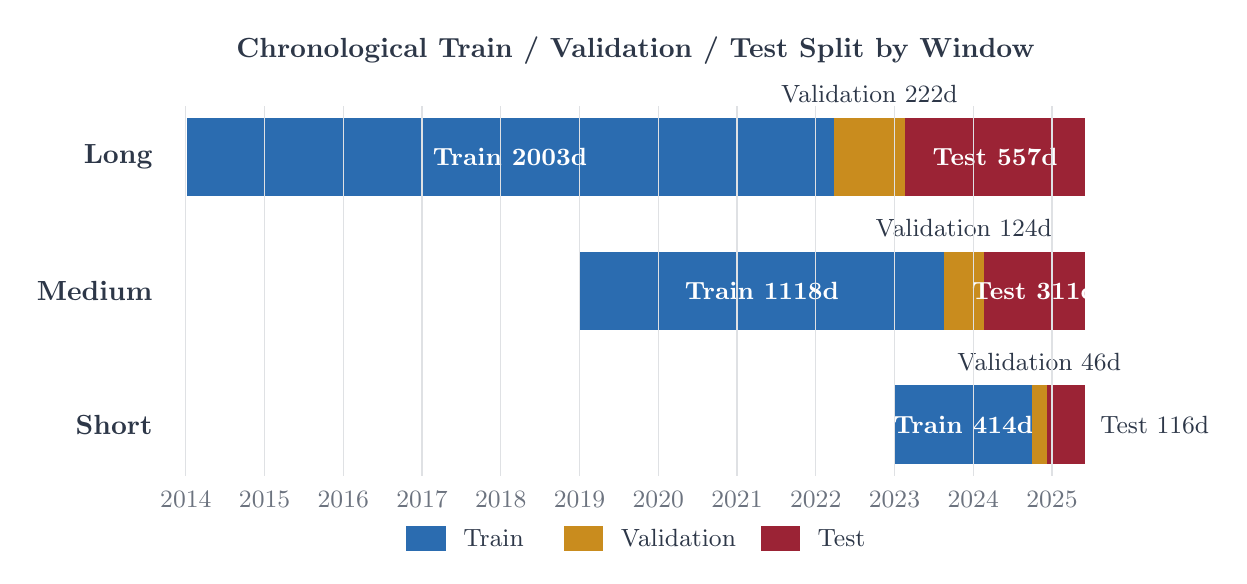
\begin{tikzpicture}[
  inlabel/.style={font=\small\bfseries, white, align=center},
  annlabel/.style={font=\small, thesisDark, align=center},
  ylabel/.style={font=\normalsize\bfseries, thesisDark, anchor=east},
  xlabel/.style={font=\small, thesisDark!70, anchor=north},
]

%% ── scale: 1 cm = 1 calendar year, origin = year 2014 ───
%% ── row height & y positions (bottom of each bar) ────────
\def\rh{1.00}     % bar height
\def\ryS{0}       % Short  row y-bottom
\def\ryM{1.7}     % Medium row y-bottom
\def\ryL{3.4}     % Long   row y-bottom

%% ── x endpoints computed from trading-day ratios ─────────
%%  Short  (2023.01–2025.42, 576d → 2.41 yr):
%%    Train 414d → 1.732yr,  Val 46d → 0.192yr,  Test 116d → 0.485yr
\def\ShX{9.01}
\def\ShTrE{10.742}  \def\ShVaE{10.934}  \def\ShEnd{11.419}

%%  Medium (2019.01–2025.42, 1553d → 6.41 yr):
%%    Train 1118d → 4.614yr, Val 124d → 0.512yr, Test 311d → 1.283yr
\def\MeX{5.01}
\def\MeTrE{9.624}   \def\MeVaE{10.136}  \def\MeEnd{11.419}

%%  Long   (2014.01–2025.42, 2782d → 11.41 yr):
%%    Train 2003d → 8.216yr, Val 222d → 0.910yr, Test 557d → 2.285yr
\def\LgX{0.01}
\def\LgTrE{8.226}   \def\LgVaE{9.136}   \def\LgEnd{11.421}

%% ── helper: draw one Gantt row ───────────────────────────
%% args: y-bot, x_start, x_trainEnd, x_valEnd, x_end
%%       trainLabel, valAnnotation, testLabel
\newcommand{\ganttrow}[8]{
  % Train bar
  \fill[thesisBlue]    (#2, {#1})   rectangle (#3, {#1+\rh});
  % Val bar
  \fill[thesisAmber]   (#3, {#1})   rectangle (#4, {#1+\rh});
  % Test bar
  \fill[thesisCrimson] (#4, {#1})   rectangle (#5, {#1+\rh});
  % Train label (inside bar, large enough)
  \node[inlabel] at ({(#2+#3)/2}, {#1+\rh/2}) {#6};
  % Val annotation (above bar, since narrow)
  \node[annlabel, above=2pt] at ({(#3+#4)/2}, {#1+\rh}) {#7};
  % Test label (inside bar if wide enough, else outside right)
  \pgfmathsetmacro{\testwidth}{(#5-#4)}
  \ifdim\testwidth cm > 1.2cm
    \node[inlabel] at ({(#4+#5)/2}, {#1+\rh/2}) {#8};
  \else
    \node[annlabel, right=2pt] at (#5, {#1+\rh/2}) {#8};
  \fi
}

%% ── Draw rows ────────────────────────────────────────────
\ganttrow{\ryL}{\LgX}{\LgTrE}{\LgVaE}{\LgEnd}
         {Train 2003d}{Validation 222d}{Test 557d}

\ganttrow{\ryM}{\MeX}{\MeTrE}{\MeVaE}{\MeEnd}
         {Train 1118d}{Validation 124d}{Test 311d}

\ganttrow{\ryS}{\ShX}{\ShTrE}{\ShVaE}{\ShEnd}
         {Train 414d}{Validation 46d}{Test 116d}

%% ── Y-axis row labels ────────────────────────────────────
\node[ylabel] at (-0.3, {\ryL+\rh/2}) {Long};
\node[ylabel] at (-0.3, {\ryM+\rh/2}) {Medium};
\node[ylabel] at (-0.3, {\ryS+\rh/2}) {Short};

%% ── X-axis year ticks + grid lines ──────────────────────
\foreach \yr in {2014,2015,...,2025}{
  \pgfmathsetmacro{\xp}{(\yr-2014)*1}
  \draw[thesisDark!15, thin] (\xp, -0.15) -- (\xp, {3.4+\rh+0.15});
  \node[xlabel] at (\xp, -0.22) {\yr};
}

%% ── Title ────────────────────────────────────────────────
\node[font=\normalsize\bfseries, thesisDark, anchor=south]
     at ({11.42/2}, {3.4+\rh+0.55})
     {Chronological Train / Validation / Test Split by Window};

%% ── Legend ───────────────────────────────────────────────
\def\legx{2.8}
\def\legy{-1.1}
\fill[thesisBlue]   (\legx, \legy) rectangle ({\legx+0.5}, {\legy+0.32});
\node[font=\small, thesisDark, anchor=west] at ({\legx+0.6}, {\legy+0.16}) {Train};
\fill[thesisAmber]  ({\legx+2.0}, \legy) rectangle ({\legx+2.5}, {\legy+0.32});
\node[font=\small, thesisDark, anchor=west] at ({\legx+2.6}, {\legy+0.16}) {Validation};
\fill[thesisCrimson]({\legx+4.5}, \legy) rectangle ({\legx+5.0}, {\legy+0.32});
\node[font=\small, thesisDark, anchor=west] at ({\legx+5.1}, {\legy+0.16}) {Test};

\end{tikzpicture}
\end{document}
